\chapter{Relationship between modified power coefficient and modified thrust coefficient}\label{ch:app_adm}

Due to present-day computational constraints, state of the art wind-farm LES grids in pseudo-spectral codes are limited to $\approx$ 10 gridpoints across the turbine diameter. As illustrated below, the use of actuator disk models for wind turbines in these resolutions lead to overpredictions in turbine power production (see, e.g., \citealp{martinez2016wind, martinez2015large}). Reviewing the expression for the disk-averaged velocity from Section \ref{sec:meth_adm}, 

\begin{align}
%\blds{f}_i(\blds{x}) &= - \frac{1}{2} \widehat{C}_{T,i}' V_{d,i}^2 \mathscr{R}_i (\blds{x}) \blds{e}_\perp,\\
%P_i(t) &= - \frac{1}{2} C_{P,i}'(t)~V_{d,i}^3(t)~A_i.\\
V_i(t) &= \frac{1}{A} \int_{\Omega} \mathscr{R}_i(\blds{x})~\ufilt \cdot \blds{e}_\perp~\dx
\end{align}
it can be shown that the main culprit in this overprediction is the geometric footprint $\mathscr{R}_i$. The diffuse smearing of the rotor geometry on the LES grid, which is required for numerical stability, leads to an overestimation of the disk velocity $V_{i}$ due to the spillover over the rotor disk region illustrated in Figure~\ref{fig:Rkernel}. This in turn entails an overprediction in power production compared to momentum theory. Note that this overprediction is not unique to actuator disk models, also in actuator line models overpredictions in turbine power are observed, for which a heuristic blade tip correction is often applied \citep{martinez2016wind}.

Figure \ref{fig:fit} illustrates $C_P$ as a function of $\widehat{C}_T'$, obtained from a steady-state actuator disk under uniform inflow. The circle markers ($\circ$) indicate simulation results with $C_P' = \widehat{C}_T'$ for the same resolution employed for the optimal induction control cases from Chapter \ref{ch:opt_induction}, and show a power coefficient $C_P$ that is too large compared to theory. Consistent with the fact that the overprediction in power is caused by an overestimation in disk velocity due to the diffuse rotor representation, the error increases for increasing $\widehat{C}_T'$, since velocity gradients are higher for larger thrust forces. Although it is shown that this overprediction is diminished for higher grid resolutions ($\triangle$), this is not a practical solution since present-day computational constraints do not allow optimal control simulations on finer grids. Therefore, a solution to this problem is to calibrate $C_P'$ based on a least-squares fit to results obtained from 1D momentum theory, yielding $C_P' = a \widehat{C}_T'$, with $a = 0.9$. From the figure it can be seen ($\square$) that this improves the $C_P$ values significantly, and that the Betz theory is now well matched. Physically, this implies that 10\% of the power depleted from the boundary layer due to the turbine presence is not captured by the rotor, but can be ascribed to dissipation losses. Remark that the coefficient $a$ depends on the simulation grid, and will tend to a value of 1 for finer and finer grids. It is worth noting that, since the proposed fit is linear, introducing a $C_P'$ differing from $\widehat{C}_T'$ eventually boils down to a postprocessing step, and does not influence the optimization itself. In other words, the actual results on power increase reported in this paper, which are all non-dimensionalized by a reference power, are not affected by the value of $a$.


\begin{figure}[h!]
	\centering
	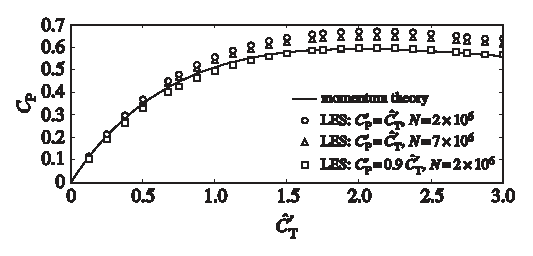
\includegraphics[width=0.8\linewidth]{chapters/appendix_adm/fig_tuning.eps}
	\caption{Power coefficient $C_P$ as a function of time-filtered modified thrust coefficient $\widehat{C}_T'$ for a steady turbine in uniform inflow.}
	\label{fig:fit}
\end{figure}

\cleardoublepage